%
% Copyright (C) 2014-2016 by Thomas Auzinger <thomas@auzinger.name>

\documentclass[draft,final]{vutinfth} % Remove option 'final' to obtain debug information.

% Load packages to allow in- and output of non-ASCII characters.
\usepackage{lmodern}        % Use an extension of the original Computer Modern font to minimize the use of bitmapped letters.
\usepackage[T1]{fontenc}    % Determines font encoding of the output. Font packages have to be included before this line.
\usepackage[utf8]{inputenc} % Determines encoding of the input. All input files have to use UTF8 encoding.

% Extended LaTeX functionality is enables by including packages with \usepackage{...}.
\usepackage{fixltx2e}   % Provides fixes for several errors in LaTeX2e.
\usepackage{amsmath}    % Extended typesetting of mathematical expression.
\usepackage{amssymb}    % Provides a multitude of mathematical symbols.
\usepackage{mathtools}  % Further extensions of mathematical typesetting.
\usepackage{microtype}  % Small-scale typographic enhancements.
\usepackage{enumitem}   % User control over the layout of lists (itemize, enumerate, description).
\usepackage{multirow}   % Allows table elements to span several rows.
\usepackage{booktabs}   % Improves the typesettings of tables.
\usepackage{subcaption} % Allows the use of subfigures and enables their referencing.
\usepackage{placeins}
\usepackage[ruled,linesnumbered,algochapter]{algorithm2e} % Enables the writing of pseudo code.
\usepackage[usenames,dvipsnames,table]{xcolor} % Allows the definition and use of colors. This package has to be included before tikz.
\usepackage{nag}       % Issues warnings when best practices in writing LaTeX documents are violated.
\usepackage{hyperref}  % Enables cross linking in the electronic document version. This package has to be included second to last.
\usepackage[acronym,toc]{glossaries} % Enables the generation of glossaries and lists fo acronyms. This package has to be included last.


% Define convenience functions to use the author name and the thesis title in the PDF document properties.
\newcommand{\authorname}{Matthias Plasser} % The author name without titles.
\newcommand{\thesistitle}{Effects of adversarial defense strategies on the decision boundary of convolutional neural networks} % The title of the thesis. The English version should be used, if it exists.
% mycommands
\newcommand{\norm}[1]{\left\lVert#1\right\rVert}

% Set PDF document properties
\hypersetup{
    pdfpagelayout   = TwoPageRight,           % How the document is shown in PDF viewers (optional).
    linkbordercolor = {Melon},                % The color of the borders of boxes around crosslinks (optional).
    pdfauthor       = {\authorname},          % The author's name in the document properties (optional).
    pdftitle        = {\thesistitle},         % The document's title in the document properties (optional).
    pdfsubject      = {Subject},              % The document's subject in the document properties (optional).
    pdfkeywords     = {a, list, of, keywords} % The document's keywords in the document properties (optional).
}

\setsecnumdepth{subsection} % Enumerate subsections.

\nonzeroparskip             % Create space between paragraphs (optional).
\setlength{\parindent}{0pt} % Remove paragraph identation (optional).

\makeindex      % Use an optional index.
\makeglossaries % Use an optional glossary.
%\glstocfalse   % Remove the glossaries from the table of contents.

% Set persons with 4 arguments:
%  {title before name}{name}{title after name}{gender}
%  where both titles are optional (i.e. can be given as empty brackets {}).
\setauthor{}{\authorname}{}{male}
\setadvisor{Ao.univ.Prof. Dr.}{Andreas Rauber}{}{male}

% For bachelor and master theses:
%\setfirstassistant{Pretitle}{Forename Surname}{Posttitle}{male}
%\setsecondassistant{Pretitle}{Forename Surname}{Posttitle}{male}
%\setthirdassistant{Pretitle}{Forename Surname}{Posttitle}{male}

% For dissertations:
%\setfirstreviewer{Pretitle}{Forename Surname}{Posttitle}{male}
%\setsecondreviewer{Pretitle}{Forename Surname}{Posttitle}{male}

% For dissertations at the PhD School:
%\setsecondadvisor{Pretitle}{Forename Surname}{Posttitle}{male}

% Required data.
\setaddress{Address}
\setregnumber{01627777}
\setdate{23}{01}{2020} % Set date with 3 arguments: {day}{month}{year}.
\settitle{\thesistitle}{Effects of adversarial defense strategies on the decision boundary of convolutional neural networks} % Sets English and German version of the title (both can be English or German).
%\setsubtitle{Optional Subtitle of the Thesis}{Optionaler Untertitel der Arbeit} % Sets English and German version of the subtitle (both can be English or German).

% Select the thesis type: bachelor / master / doctor / phd-school.
% Bachelor:
\setthesis{bachelor}

% For bachelor and master:
\setcurriculum{Software and Information Engineering}{Software und Information Engineering} % Sets the English and German name of the curriculum.

% For dissertations at the PhD School:
%\setfirstreviewerdata{Affiliation, Country}
%\setsecondreviewerdata{Affiliation, Country}

% Define convenience macros.
\newcommand{\todo}[1]{{\color{red}\textbf{TODO: {#1}}}} % Comment for the final version, to raise errors.


\begin{document}

\frontmatter % Switches to roman numbering.
% The structure of the thesis has to conform to
%  http://www.informatik.tuwien.ac.at/dekanat

%\addtitlepage{naustrian} % German title page (not for dissertations at the PhD School).
\addtitlepage{english} % English title page.
%\addstatementpage

\begin{abstract}
Neural Networks are more powerful than ever, but still have security-relevant weaknesses: their decision-making cannot be understood fully yet, but still be hijacked easily.
Many techniques exist for manipulating inputs for neural networks in a way to get misclassified, although to a human there is no perceptible difference to the original input.
Adversarial Examples suggest, that neural networks do not learn true universal underlying concepts from their training data, but just a concept that works on the given data distribution.
This work examines, how strategies for defending neural networks against adversarial attacks influence the decision boundary of neural networks in two experiments.
As the decision boundary of neural networks is an abstract, high dimensional hyperplane it gets examined indirectly.
One experiment examines how adversarial training enables neural networks to recognize some adversarial examples.
The second experiment visualizes how adversarial examples that are constructed for defended networks distinguish from undefended models.
Adversarial training increases a classifier's ability to recognize adversarial examples, although not nearly as many as validation examples.
Furthermore, defended models force adversarial attacks to craft inputs, that are easier distinguishable from the original input.

\end{abstract}

% Select the language of the thesis, e.g., english or naustrian.
\selectlanguage{english}

% Add a table of contents (toc).
\tableofcontents % Starred version, i.e., \tableofcontents*, removes the self-entry.

% Switch to arabic numbering and start the enumeration of chapters in the table of content.
\mainmatter

\chapter{Introduction}

\section{Overview}

Neural Networks are more reliable than ever in 2020, and outperform human experts in a broad range of tasks, from playing Go to recognizing fractures in MRIs.
The existence of adversary examples - examples that are carefully, (almost) imperceptibly manipulated in order to get misclassified by neural networks challenges that reliability.
Adversary inputs can be constructed from an input that is initially correctly labelled by a classifier.
By carefully manipulating features by a tiny amount in the correct direction - towards the decision boundary, it is possible to
craft data that to a human still appears like the original input, yet gets labeled as something else by the given classifier.
Adversarial Inputs can even be printed out, photographed, and still get misclassified in some cases.
Adversarial Examples indicate, that DNNs might not learn generalizing concepts a human could understand like looking for key features in an image, but just concepts that work well on the given data distribution, and do not rely on stable features.
Various defense techniques against adversarial examples exist.
Defending a DNN against Adversarial Attacks should not only decrease it's vulnerability, but also increase the comprehensibility for Adversarial Inputs that could successfully fool a classifier - they should also be more likely to fool a human.

\section{Aim of Work}

The aim of this work is gaining insights into the reason for the existence of Adversarial Examples and the decision boundaries and the decision process of deep neural networks.
Therefore, the effects of adversarial defense strategies - Adversarial Training and Input Gradient Regularization are examined addressing the following questions:

\textbf{To what extent can adversarial defense strategies improve the performance of different convolutional neural networks on adversarial examples?}
If adversarial defense strategies could prevent adversarial attacks from successfully finding adversarial examples, adversarial examples would only be a small threat to the reliability of CNNs.
In case adversarial defense strategies cannot fully defend classifiers against adversarial attacks, comparing the success rates of defenses for different network architectures could expose
interesting insights, which leads to the next research question:
\textbf{How does network complexity and -depth influence the defensibility against adversarial attacks?}
If adversarial defense strategies improve the accuracy of classifiers on adversarial examples, adversarial attacks should be forced to create examples, that are more similar to their target
class in order to reach misclassification.
This hypothesis is addressed by the following question:
\textbf{What effects do adversarial defense strategies have on the appearance of adversarial examples generated by adversarial attacks?}

\chapter{Fundamentals}

In this chapter some basics will be introduced in a level of detail required for comprehending the following work.
For a higher level of detail and further reading, references are provided.

\section{Adversarial Examples}

Adversarial Examples are inputs that show faults in the input-output mappings of neural networks.
Those inputs are easy to classify correctly for a human, but misclassified by a certain classifier with high confidence.
Adversarial inputs are usually generated by imperceptibly modifying existing, genuine inputs, some methods can achieve misclassification by modifying just a single pixel\cite{Jiawei2017}.
Christian Szegedy et al. were the first to describe adversarial examples for (deep) neural networks in 2013, and they suspect, that small "pockets" occuring in the input-output mappings enable the existence of adversarial examples.
They found, that adversarial examples generated for one model are also statistically hard to classify for networks with different hyperparameters, or even more surprising for networks trained on different data sets \cite{Szegedy2013}.

\section{Adversarial Attacks}
\label{section:adv_att}

This section is about the algorithms for generating adversarial examples used in the experiments of this work.
After a brief introduction and theoretical justification for the existence of Adversarial Examples, the Fast Gradient Sign Method, the Basic Iterative Method and the Single Pixel Attack will be explained.\\
Since the discovery of adversarial examples for DNNs in 2013, dozens of methods for generating them have been developed.
Adversarial Attacks can be targeted or untargeted, where the targeted version aims to make a classifier predict a certain class for an input, while an untargeted attack seeks minimization for the predicted probability of the correct class.
Furthermore, adversarial attacks can be divided in black or white box attacks, where white box attacks have access to some or all model parameters, while inference of a model's prediction is sufficient for black box attacks.
\\
The following explanation assumes linear behavior of the input-output mapping of the classifiers attacked.
In a small range around an input, this assumption holds for many different, even highly unlinear models, as they are designed and tuned to operate mostly in the linear section \cite{Goodfellow2015}.
Approximating one output function of a classifier in the local environment around an input vector $x$ with $w^T$, this activation function can be written as a dot product: $f(x) = w^Tx$.
Introducing an adversary input $\tilde{x}$ as the sum of the original input $x$ and a perturbation $\eta$, with maximal magnitude $\epsilon$, we can write the activation function for $\tilde{x}$ like follows:

\begin{equation}
	f(\tilde{x}) = w^Tx + w^T\eta
\end{equation}

For maximizing the change induced by $\eta$ in relation to its largest magnitude $\epsilon$, it is optimal to set $\eta = \epsilon sign(w)$.
The effect on the activation for $\tilde{x}$ can be calculated by $\epsilon*m*n$, where $m$ is the average magnitude of $w$, and $n$ is the number of dimensions of $w$ and the input $x$.
As $\norm{sign(w)}_\infty = 1$ is valid and invariant of the number of dimensions, but the impact of $\eta$ on $m*n$ and hence on $f(\tilde{x})$ grows linearly with $n$, classifiers are more vulnerable to adversarial inputs the higher the dimensionality of their input vectors is. \cite{Goodfellow2015}

\subsection{Fast Gradient Sign Method}

This computely very cheap method for finding adversarial examples was described by Goodfellow et al. in 2015, and relies on the assumption of linearity in a range around an input $x$.
Given model parameters $\theta$, an input $x$, the true label $y_{true}$ and the model's loss function $J$, a perturbation $\eta$ can be calculated as follows:

\begin{equation}
	\eta = \epsilon sign(\nabla_xJ(\theta, x, y_{true}))
\end{equation}

$\eta$ can be considered to "follow" the gradient of the loss function in respect of the input, and thus to change the loss function in an optimal way in relation to its maximal magnitude $\norm{\eta}_\infty$.
\\
Hence, this untargeted form of the Fast Gradient Sign Method works by maximizing the loss function for the given input and its true label.
Therefore, a targeted version of the attack can be obtained by minimizing the loss function for the current input and the taget label $y_{target}$:

\begin{equation}
	\eta = -\epsilon sign(\nabla_xJ(\theta, x, y_{target}))
\end{equation}
\cite{Goodfellow2015}

\subsection{Basic Iterative Method}

As a straightforward extension to the Fast Gradient Sign Method, the Basic Iterative Method does not perturb the original input in a single step with width $\epsilon$, but iteratively applies smaller changes. As in each iteration the gradient is evaluated anew, this method can follow the gradient more accurately, and therefore may require a smaller maximal magnitude of the perturbation. The untargeted version of the Basic Iterative Method can be formulated in the following way:

\begin{equation}
	X^{adv}_0 = X, X^{adv}_{N+1} = Clip_{X,e}\{X^{adv}_{N} + \alpha sign(\nabla_xJ(X^{adv}_{N}, y_{true})) \}
\end{equation}

$\alpha$ limits the step size per iteration, while $\epsilon$ still constrains the maximal magnitude of difference between the final adversarial image and the orignal input.

\subsection{One Pixel Attack}

The Single Pixel Attack is an extremely limited method for finding adversarial examples.
Instead of limiting the magnitude of the perturbation, its dimensionality is constrained to be 1 ($\norm{\eta}_0=1$).
Jiawei Su et al. describe a way for finding single pixel modifications that lead to misclassification by differential evolution.
This algorithm works by maintaining an amount of candidate solutions (400), combining their features and selecting the fittest among the parent and child generations.
The only information this method requires from the attacked classifier is the output-probabilities, so the One Pixel Attack is a black box attack, and also not reliant on gradients \cite{Jiawei2017}.
As this method works entirely different than the Fast Gradient Sign Method, it is ideal for evaluating adversarial robustness of a model after adversarial training using FGSM.

\section{Adversarial Defenses}

Since the discovery of adversarial attacks, also defenses against them have been developed.
In this section the two adversarial defense strategies used in the experiments of this work will be described briefly.

\subsection{Adversarial Training}

Goodfellow et al. suggest using adversarial inputs for training to gain adversarial robustness.
The Fast Gradient Sign Method is very convenient for adversarial training, as it is computely cheap, and can be integrated in the loss function:

\begin{equation}
	\label{eq:adv_loss}
	\tilde{J}(\theta, x, y_{true}) = \alpha J(\theta, x, y_{true}) + (1-\alpha)J(\theta, x + \epsilon sign(\nabla_xJ(\theta, x, y_{true})), y_{true})
\end{equation}

Minimizing the adversarial loss function $\tilde{J}(\theta, x, y_{true})$ means not only optimizing the loss for the training samples, but also for adversarial examples crafted from the training set.
\cite{Goodfellow2015}

\subsection{Input Gradient Regularization}

Another way of gaining adversarial robustness was proposed by Andrew Slavin Ross and Finale Doshi-Velez: if not only a model's accuracy, but also the rate of change in respect to the inputs is minimized, small changes to the input should not be able to lead to significant changes in the output. 
Input Gradient Regularization can, like adversarial training be achieved by modifying the loss function J:

\begin{equation}
	\tilde{J}(\theta, x, y_{true}) = J(\theta, x, y_{true}) + \lambda \norm{(\nabla_x J(\theta, x, y_{true}))}_2^2
	\label{eq:gradreg}
\end{equation}

The parameter $\lambda$ determines, how strong the input gradient is weighed compared to the initial loss, and has to be tuned individually, as it is highly dependent on many hyperparameters of the classifier \cite{Ross2017}.

\section{Decision Boundary}

The decision boundary of neural networks is a hyperplane in their input space and separates classes distinguised by the classifier.
Thus, typical classifiers being able to discriminate among more than two classes possess multiple decision boundaries.
The shape of the decision boundary exposes interesting properties about the decision process: the smoother and simpler it is, the more stable a prediction made is.\\
Back in 1200s William of Ockham formulated his law of parsimony, also known as occam’s razor, which states, that everything else being equal, the simplest explanation is the most likely. 
How this translates to machine learning is not very clear, but still it can be shown for some learning problems, that solutions that require a shorter explanation in any bit-wise representation perform better than longer explanations \cite{Blumer1987}.\\
As the decision boundary of DNNs is encoded into the weights, the length of their bit-wise representation is constant, but it is still intuitive, that simpler, smoother decision-boundaries provide predictions that are more stable, especially when recalling the explanation for the existence of Adversarial Examples.

\section{Grad-CAM++}

Grad-CAM++ is a progression and generalization of Grad-CAM, a visual approach of explaining decisions of CNNs using gradient weighted class activation maps.
Grad-CAM++ highlights features of an image, that were most important for a CNNs decision on the image (see \ref{fig:exp:iat:heatmap}).
As spatial locality is preserved in feature maps ($A$) of CNNs, the importance of a location $i j$ for class $c$ can be written as:

\begin{equation}
	L_{ij}^c = \sum_{k} w_k^c * A^k
\end{equation}

The difference between CAM, Grad-CAM and Grad-CAM++ lies in the determination of $w_k^c$, the weight of the $k^{th}$ feature map.
In Grad-CAM++ $w_k^c$ is calculated as follows, where $Y^c$ denotes the output activation for class $c$ (sum over all spatial locations), $relu$ is the rectified linear unit function

\begin{equation}
	w_k^c = \sum_i \sum_j \alpha_{ij}^{kc} * relu(\frac{\partial Y^c}{\partial A_{ij}^k})
\end{equation}

$\alpha_{ij}^{kc}$ are weighting coefficients, that make sure the presence of objects in feature maps are highlighted with equal importance regardless of their activation.
The reason the $relu$ function is used is, that only features that increase the desired output are meaningful in a visualization.
\cite{Chattopadhyay2017}
\label{section:grad_cam}

\chapter{Related Work}

This chapter will briefly summarize publications that are similar to this work, or contain fundamentals for it, and state, how this publications are relevant for this work.

\section{Intriguing properties of neural networks}

Intentionally crafted adversarial examples for deep neural networks were first described by Christian Szegedy et al. in 2013 \cite{Szegedy2013}.
They conclude, that although (deep) neural networks are thought to achieve high generalization, they show discontinuities in their input-output mappings, which enable the existence of adversarial inputs.
The authors also propose the L-BFGS method for finding adversarial examples, and suggest using this method for hard negative mining and generating valuable training data.
Theoretical insights of this paper were used in the Fundamentals section.\\
%Warren He et al. examined decision boundaries around adversarial images.
%They introduced an adversarial attack method able to evade common adversarial defense techniques, like adversarial training.
%Furthermore, He et al. found examining the distance of input samples from decision boundaries could reveal differences between adversarial and benign inputs \cite{He2018}.
%However, they did not visualize the decision boundary of the networks they trained in form of class-activation maps nor heat-maps.\\
\section{Grad-CAM++: Improved Visual Explanations for Deep Convolutional Networks}
Chattopadhyay, Sarkar et al. proposed the method of visualizing, what areas of an image appear especially important for image classification to convolutional neural networks used in the first experiment of this work. 
Due to the fact, that spatial information is preserved in the convolutional layers of CNNs, and the ability to calculate the gradient between outputs of the last convolutional layer and the desired output, weights can be assigned to all parts of the input image.
Weighing the localizable activations in the last convolutional layer of a CNN results in a map, that highlights the areas of greatest importance for the made prediction \cite{Chattopadhyay2017}.
\section{Improving the Adversarial Robustness and Interpretability of Deep Neural Networks by Regularizing their Input Gradients}
Ross and Doshi-Velez proposed, that the uninterpretability and adversarial vulnerability of deep neural networks are mutually dependent.
As in image classification tasks noisy input gradients are often very difficult to interpret, the authors hypothesize, that regularizing (minimizing) those gradients should not only improve the interpretability, but also the Adversarial Robustness of a classifier.
What supports their hypothesis is, that many adversarial attacks rely on input gradients.
In their experiments, in addition to being able to confirm their hypothesis, the authors also found, that adversarial examples that successfully fooled a classifier with regularized input gradients also could fool a human, as those examples were more similar to their target class than to their original label.
The experiments of this work, also utilize Input Gradient Regularization, and Adversarial Examples are presented in way similar to the "confusion-matrices" Ross and Dosi-Velez showed \cite{Ross2017}.



\chapter{Methodology}

This chapter will in describe how the experiments of this work were performed, and how they expose information about the decision boundary.\\

In the experiment, different network architectures are trained using different defense strategies: adversarial training, input gradient regularization and a combination of both.
As decision-boundaries in 12,288 (=$64*64*3$) dimensions might be challenging to visualize and grasp, their shape is studied in indirect ways.\\
In both experiments Categorical Crossentropy is used as loss function, and training is done over 10 epochs for all network architectures.
The learning rate is 0.001 for the first 9 epochs, and decreased to 0.0001 only in the last epoch.
The first experiment examines the effects of Adversarial Training on the decision boundaries in terms of accuracy iteratively.
Additionally, in the first experiment heatmaps that highlight most important areas for the classification of an image are created, for comparison.
The second experiment examines the appearance of Adversarial Examples, as the decision boundary lies between the original input and the perturbed one.

\section{Training Data}

The German Traffic Sign Recognition Benchmark is used as original training data. The set consists of 39209 labeled 64x64 RGB images for training, and 12630 for validation.
The images are distributed unevenly among the classes, and contain little distortions.


\section{Neural Network Architectures}

Several architectures of CNNs are considered, as varying architectures, and especially depths may have an effect on adversarial vulnerability.
The following table lists the used networks with their corresponding depths and numbers of trainable parameters:

\begin{table}[h]
  \centering
  \begin{tabular}{cccc}
    \toprule
		Name    		& Depth		& Trainable Parameters\\
    \midrule
		lenet-5			&	8				& 391,307							\\
		alexnet 		& 16			& 2,668,875						\\
		VGG19				& 25			& 21,611,307					\\
		ResNet50		& 178			& 32,021,419					\\
    
    \bottomrule
  \end{tabular}
\end{table}


The VGG19 and the ResNet are not fully trained from scratch, but already pretrained on ImageNet.

\section{Implementation}

The implementation of the experiments is done in python 3.5 using Tensorflow, Keras and Cleverhans.
For verification and reproducibility, the source code of the experiments is available on github: \url{https://github.com/plassma/GTSRB-adversarial-training}
Parts of the program were copied from a Keras Model demo Maximilian Idahl published on github under the MIT license \cite{Idahl2018}.
As malicious versions or wrong combinations of Tensorflow and cuDNN versions often led to problems, a version-table of the most important frameworks used is included:

\section{Frameworks}

\begin{table}[h]
  \centering
  \begin{tabular}{cl}
    \toprule
		Name                                & Version   \\
    \midrule
    Numpy                               & 16.16.6	  \\
    Tensorflow                          & 1.14.0    \\
    Tensorflow-GPU                      & 1.14.0    \\
    Keras                               & 2.3.1     \\
    Adversarial-Robustness-Toolkit      & 1.0.1     \\
    Cleverhans                          & 3.0.1     \\
    Foolbox                             & 2.3.0     \\
		cuDNN																&	7.6.5			\\
		NVIDIA WHQL													& 441.66		\\
		
    
    \bottomrule
  \end{tabular}
\end{table}


\chapter{Experiment - Iterative Adversarial Training}
In this chapter the first experiment and its results will be described and discussed in detail.

\section{Description}

In this experiment adversary training is performed iteratively, each iteration consisting of some evaluation steps and a run of adversary training.
Two modes of training are distinguished: in one mode no defenses are applied, while in the other the loss function is modified to weigh Adversarial Loss with $\alpha = 0.5$ (see Equation \ref{eq:adv_loss}).
In each iteration Adversary Inputs are generated from the validation set using untargeted FGSM with $\epsilon = 0.05$.
The Adversary Input sets do not get filtered, and contain actual Adversary Inputs as well as Inputs that still get classified correctly.
The accuracies on those Adversary Sets are considered proportional to the Adversary Robustness of a classifier.
The model is then trained for an epoch, and its accuracy is evaluated not only against the validation- and the current Adversary Input set, but also against all preceding Adversary Input sets, before the next iteration begins.
Additionally, heatmaps (see \ref{section:grad_cam}) that expose what areas of an input were most important for the model's decision are created for some inputs from the validation set and the current Adversary input set before and after the Adversary Training.
A shift of areas that were most important for an image's classification is expected towards features that appear like key features to a human.

\section{Results}

\subsection{lenet-5}

\begin{figure}[h]
  \begin{subfigure}[b]{0.5\columnwidth}
		\centering
    \includegraphics[width=\textwidth]{Results/iterative_adversarial_training/lenet-5/standard_loss}
    \subcaption{Accuracies with undefended loss}
    \label{fig:exp:iat:lenet-5:data}
  \end{subfigure}
  \begin{subfigure}[b]{0.5\columnwidth}
		\centering
    \includegraphics[width=\textwidth]{Results/iterative_adversarial_training/lenet-5/adv_loss}
    \subcaption{Accuracies with Adversarial loss}
    \label{fig:exp:iat:lenet-5:loss}
  \end{subfigure}
  \caption{Accuracies of lenet-5 in iterative Adversarial Training}
\end{figure}

\begin{figure}[h]
	\begin{subfigure}[b]{0.5\columnwidth}
		\centering
    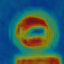
\includegraphics[width=\textwidth]{Results/iterative_adversarial_training/heatmaps/normal_0}
    \subcaption{Heatmap of undefended lenet-5 in \hspace{\textwidth} iteration 1}
    \label{fig:exp:iat:lenet-5-heat:normal_0}
  \end{subfigure}
  \begin{subfigure}[b]{0.5\columnwidth}
		\centering
    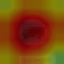
\includegraphics[width=\textwidth]{Results/iterative_adversarial_training/heatmaps/normal_1}
    \subcaption{Heatmap of undefended lenet-5 in \hspace{\textwidth} iteration 10}
    \label{fig:exp:iat:lenet-5-heat:normal_1}
  \end{subfigure}

	\begin{subfigure}[b]{0.5\columnwidth}
		\centering
    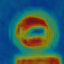
\includegraphics[width=\textwidth]{Results/iterative_adversarial_training/heatmaps/adv_0}
    \subcaption{Heatmap of adversarially trained lenet-5 in iteration 1}
    \label{fig:exp:iat:lenet-5-heat:adv_0}
  \end{subfigure}
  \begin{subfigure}[b]{0.5\columnwidth}
		\centering
    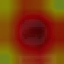
\includegraphics[width=\textwidth]{Results/iterative_adversarial_training/heatmaps/adv_1}
    \subcaption{Heatmap of adversarially trained lenet-5 in iteration 10}
    \label{fig:exp:iat:lenet-5-heat:adv_1}
  \end{subfigure}
  \caption{Heatmaps for lenet-5 correctly classifying 'Vehicles over 3.5 metric tons prohibited'}
	\label{fig:exp:iat:heatmap}
\end{figure}

\FloatBarrier

\subsection{alexnet}

\begin{figure}[h]
  \begin{subfigure}[b]{0.5\columnwidth}
		\centering
    \includegraphics[width=\textwidth]{Results/iterative_adversarial_training/alex/standard_loss}
    \subcaption{Accuracies with undefended loss}
    \label{fig:exp:iat:alex:data}
  \end{subfigure}
  \begin{subfigure}[b]{0.5\columnwidth}
		\centering
    \includegraphics[width=\textwidth]{Results/iterative_adversarial_training/alex/adv_loss}
    \subcaption{Accuracies with Adversarial loss}
    \label{fig:exp:iat:alex:loss}
  \end{subfigure}
  \caption{Accuracies of alexnet in iterative Adversarial Training}
\end{figure}

\FloatBarrier
\subsection{vgg19}

\begin{figure}[h]
  \begin{subfigure}[b]{0.5\columnwidth}
		\centering
    \includegraphics[width=\textwidth]{Results/iterative_adversarial_training/vgg19/standard_loss}
    \subcaption{Accuracies with undefended loss}
    \label{fig:exp:iat:alex:data}
  \end{subfigure}
  \begin{subfigure}[b]{0.5\columnwidth}
		\centering
    \includegraphics[width=\textwidth]{Results/iterative_adversarial_training/vgg19/adv_loss}
    \subcaption{Accuracies with Adversarial loss}
    \label{fig:exp:iat:alex:loss}
  \end{subfigure}
  \caption{Accuracies of vgg19 in iterative Adversarial Training}
\end{figure}

\FloatBarrier
\subsection{resnet-50}

Unfortunately, the experiment could not be performed for the resnet-50, as the accuracy did not rise above 0.05.
After correct behavior of the network in training during the first few batches, the loss starts to increase again.
The reason for this probably lies in the high complexity of the adversarial loss function and memory issues during training.

\section{Discussion}


For every architecture, Adversarial Training clearly does increase the robustness for FGSM attacks, while maintaining the validation accuracy.
The adversary accuracies are consistently increased for all Adversary Input sets generated during the experiment, which means that the classifiers actually learn to recognize
Adversary Inputs, and not to 'hide' them from FGSM while still being vulnerable to them.
It seems like more complex networks are more adversarially robust, although that cannot be concluded by comparing the performance of 3 architectures.\\

No significant effects of adversarial training on heatmaps could be examined.
This is plausible, when recalling the linear explanation for the existence of Adversarial Inputs (\ref{section:adv_att}).
The adversarial robustness is not a result of focusing on more stable features, but probably arises from eliminating some 'pockets' in the decision boundary.


\chapter{Experiment - Confusion Matrix}

In this chapter the second experiment and its results will be described and discussed in detail.

\section{Description}
This experiment is about visualizing the decision-boundary indirectly through Adversarial Inputs that are generated by iterative targeted FGSM.
Targeted FGSM modifies inputs in the direction of the closest decision boundary.
By examining the appearance of those Adversarials, conclusions about the decision boundary can be made.
In this experiment, models are trained with different defense strategies: none, Adversarial Training using FGSM, Input Gradient Regularization and a combination of the latter two techniques.
These trained models will be attacked using the targeted Basic Iterative Method, in one attempt targets will be very similar to the original label, in the other they will be very distinctive.
The results of the attack - the Adversarial images are ordered in a matrix.
Each column has the same attack target, while each row consists of the same original input - the determinant depicts the original inputs.
A table containing accuracies and defense parameters for each combination of network architecture and defense strategy is given.
$\alpha$ and $\epsilon$ FGSM stand for the weight of the adversarial loss and the maximal perturbation of Adversarial Inputs in the adversarial training loss function \ref{eq:adv_loss}, while $\lambda$ denotes the regularization-coefficient from \ref{eq:gradreg}. $\lambda$ was chosen heuristically and set to a value that did not decrease the validation accuracy much, while having a decreasing effect on the Input Gradient.
Additionally, the average and maximal input gradient among the validation-set is given.
All combinations of architecture and defense strategy where trained for 10 epochs, except the lenet-5 which was trained for 20 epochs.
The learning rate was 0.001 for the first 9 epochs and 0.0001 afterward for all combinations.


\section{Results}

The following sections contain the results of the experiment, each heading for a different combination of model and defense strategy.


\subsection{lenet-5 with no defenses implemented}

\begin{table}[h]
  \centering
  \begin{tabular}{ll}
    \toprule
			Parameter			& Value   \\
    \midrule
			$\lambda$								& 0				\\
			$\alpha$								& 0				\\
			$\epsilon$ FGSM					& 0.05		\\
			Epochs training					& 20			\\
			
			Validation Accuracy			& 0.892		\\ 
			Adv Accuracy - FGSM			& 0.200		\\
%			Adv Accuracy - SPA			& 0.898		\\
			
			Avg Input Gradient			& 20.799	\\
			Max Input Gradient			& 6521.212\\
    \bottomrule
  \end{tabular}
\end{table}


\begin{figure}[h]
  \begin{subfigure}[b]{0.5\columnwidth}
		\centering
    \includegraphics[width=\textwidth]{Results/confusion_matrix/lenet-5/similar}
    \subcaption{Targeted BIM for similar Images}
    \label{fig:exp:cm:lenet-5:similar}
  \end{subfigure}
  \begin{subfigure}[b]{0.5\columnwidth}
		\centering
    \includegraphics[width=\textwidth]{Results/confusion_matrix/lenet-5/different}
    \subcaption{Targeted BIM for different Images}
    \label{fig:exp:cm:lenet-5:different}
  \end{subfigure}
  \caption{Targeted Basic Iterative Method on lenet-5 with no defenses}
  \label{fig:exp:cm:lenet-5}
\end{figure}
\clearpage

\subsection{lenet-5 with Input Gradient Regularization}

\begin{table}[h]
  \centering
  \begin{tabular}{ll}
    \toprule
			Parameter			& Value   					\\
    \midrule
			$\lambda$								& 0.4			\\
			$\alpha$								& 0				\\
			$\epsilon$ FGSM					& 0.05		\\
			Epochs training					& 20			\\
			
			Validation Accuracy			& 0.760		\\ 
			Adv Accuracy - FGSM			& 0.194		\\
%			Adv Accuracy - SPA			& 0.898		\\
			
			Avg Input Gradient			& 8.620		\\
			Max Input Gradient			& 411.353	\\
    \bottomrule
  \end{tabular}
\end{table}


\begin{figure}[h]
  \begin{subfigure}[b]{0.5\columnwidth}
		\centering
    \includegraphics[width=\textwidth]{Results/confusion_matrix/lenet-5_gradreg/similar}
    \subcaption{Targeted BIM for similar Images}
    \label{fig:exp:cm:lenet-5_gradreg:similar}
  \end{subfigure}
  \begin{subfigure}[b]{0.5\columnwidth}
		\centering
    \includegraphics[width=\textwidth]{Results/confusion_matrix/lenet-5_gradreg/different}
    \subcaption{Targeted BIM for different Images}
    \label{fig:exp:cm:lenet-5_gradreg:different}
  \end{subfigure}
  \caption{Targeted Basic Iterative Method on lenet-5 with Input Gradient Regularization}
  \label{fig:exp:cm:lenet-5_gradreg}
\end{figure}
\clearpage

\subsection{lenet-5 with Adversarial Training}

\begin{table}[h]
  \centering
  \begin{tabular}{ll}
    \toprule
			Parameter			& Value   \\
    \midrule
			$\lambda$								& 0				\\
			$\alpha$								& 0.5			\\
			$\epsilon$ FGSM					& 0.05		\\
			Epochs training					& 20			\\
			
			Validation Accuracy			& 0.816		\\ 
			Adv Accuracy - FGSM			& 0.405		\\
			%Adv Accuracy - SPA			& 0.898		\\
			
			Avg Input Gradient			& 22.584	\\
			Max Input Gradient			& 2281.173\\
    \bottomrule
  \end{tabular}
\end{table}


\begin{figure}[h]
  \begin{subfigure}[b]{0.5\columnwidth}
		\centering
    \includegraphics[width=\textwidth]{Results/confusion_matrix/lenet-5_adv/similar}
    \subcaption{Targeted BIM for similar Images}
    \label{fig:exp:cm:lenet-5_adv:similar}
  \end{subfigure}
  \begin{subfigure}[b]{0.5\columnwidth}
		\centering
    \includegraphics[width=\textwidth]{Results/confusion_matrix/lenet-5_adv/different}
    \subcaption{Targeted BIM for different Images}
    \label{fig:exp:cm:lenet-5_adv:different}
  \end{subfigure}
  \caption{Targeted Basic Iterative Method on lenet-5 with Adversarial Training}
  \label{fig:exp:cm:lenet-5_adv}
\end{figure}
\clearpage

\subsection{lenet-5 with Adversarial Training and Input Gradient Regularization}

\begin{table}[h]
  \centering
  \begin{tabular}{ll}
    \toprule
			Parameter			& Value   \\
    \midrule
			$\lambda$								& 0.4			\\
			$\alpha$								& 0.5			\\
			$\epsilon$ FGSM					& 0.05		\\
			Epochs training					& 20			\\
			
			Validation Accuracy			& 0.766		\\ 
			Adv Accuracy - FGSM			& 0.400		\\
			%Adv Accuracy - SPA			& 0.898		\\
			
			Avg Input Gradient			& 13.832	\\
			Max Input Gradient			& 521.101	\\
    \bottomrule
  \end{tabular}
\end{table}


\begin{figure}[h]
  \begin{subfigure}[b]{0.5\columnwidth}
		\centering
    \includegraphics[width=\textwidth]{Results/confusion_matrix/lenet-5_gradreg_adv/similar}
    \subcaption{Targeted BIM for similar Images}
    \label{fig:exp:cm:lenet-5_gradreg_adv:similar}
  \end{subfigure}
  \begin{subfigure}[b]{0.5\columnwidth}
		\centering
    \includegraphics[width=\textwidth]{Results/confusion_matrix/lenet-5_gradreg_adv/different}
    \subcaption{Targeted BIM for different Images}
    \label{fig:exp:cm:lenet-5_gradreg_adv:different}
  \end{subfigure}
  \caption{Targeted Basic Iterative Method on lenet-5 with Adversarial Training and Input Gradient Regularization}
  \label{fig:exp:cm:lenet-5_gradreg_adv}
\end{figure}
\clearpage


\subsection{Alexnet with no defenses implemented}

\begin{table}[h]
  \centering
  \begin{tabular}{ll}
    \toprule
			Parameter			& Value   \\
    \midrule
			$\lambda$								& 0				\\
			$\alpha$								& 0				\\
			$\epsilon$ FGSM					& 0.05		\\
			Epochs training					& 10			\\
			
			Validation Accuracy			& 0.961		\\
			Adv Accuracy - FGSM			& 0.342		\\
			%Adv Accuracy - SPA			& 0.898		\\
			
			Avg Input Gradient			& 21.575	\\
			Max Input Gradient			& 7156.949\\
    \bottomrule
  \end{tabular}
\end{table}


\begin{figure}[h]
  \begin{subfigure}[b]{0.5\columnwidth}
		\centering
    \includegraphics[width=\textwidth]{Results/confusion_matrix/alex/similar}%eps=0.01, iter=15
    \subcaption{Targeted BIM for similar Images}
    \label{fig:exp:cm:alex:similar}
  \end{subfigure}
  \begin{subfigure}[b]{0.5\columnwidth}
		\centering
    \includegraphics[width=\textwidth]{Results/confusion_matrix/alex/different}
    \subcaption{Targeted BIM for different Images}
    \label{fig:exp:cm:alex:different}
  \end{subfigure}
  \caption{Targeted Basic Iterative Method on alexnet with no defenses}
	\label{fig:exp:cm:alex}
\end{figure}
\clearpage

\subsection{Alexnet with Input Gradient Regularization}

\begin{table}[h]
  \centering
  \begin{tabular}{ll}
    \toprule
			Parameter			& Value   \\
    \midrule
			$\lambda$								& 0.15		\\
			$\alpha$								& 0				\\
			$\epsilon$ FGSM					& 0.05		\\
			Epochs training					& 10			\\
			
			Validation Accuracy			& 0.949		\\
			Adv Accuracy - FGSM			& 0.375		\\
			%Adv Accuracy - SPA			& 0.922		\\
			
			Avg Input Gradient			& 2.926		\\
			Max Input Gradient			& 520.662 \\
    \bottomrule
  \end{tabular}
\end{table}


\begin{figure}[h]
  \begin{subfigure}[b]{0.5\columnwidth}
		\centering
    \includegraphics[width=\textwidth]{Results/confusion_matrix/alex_gradreg/similar}%eps=0.01, iter=15
    \subcaption{Targeted BIM for similar Images}
    \label{fig:exp:cm:alex_gradreg:similar}
  \end{subfigure}
  \begin{subfigure}[b]{0.5\columnwidth}
		\centering
    \includegraphics[width=\textwidth]{Results/confusion_matrix/alex_gradreg/different}
    \subcaption{Targeted BIM for different Images}
    \label{fig:exp:cm:alex_gradreg:different}
  \end{subfigure}
  \caption{Targeted Basic Iterative Method on alexnet with Input Gradient Regularization}
\end{figure}
\clearpage

\subsection{Alexnet with Adversarial Training}
\begin{table}[h]
  \centering
  \begin{tabular}{ll}
    \toprule
			Parameter			& Value   \\
    \midrule
			$\lambda$								& 0				\\
			$\alpha$								& 0.5			\\
			$\epsilon$ FGSM					& 0.05		\\
			Epochs training					& 10			\\
			
			Validation Accuracy			& 0.947		\\
			Adv Accuracy - FGSM			& 0.633 	\\
			%Adv Accuracy - SPA			& 0.898		\\
			
			Avg Input Gradient			& 34.878	\\
			Max Input Gradient 			& 4473.322\\
    \bottomrule
  \end{tabular}
\end{table}


\begin{figure}[h]
  \begin{subfigure}[b]{0.5\columnwidth}
		\centering
    \includegraphics[width=\textwidth]{Results/confusion_matrix/alex_adv/similar}
    \subcaption{Targeted BIM for similar Images}
    \label{fig:exp:cm:alex_adv:similar}
  \end{subfigure}
  \begin{subfigure}[b]{0.5\columnwidth}
		\centering
    \includegraphics[width=\textwidth]{Results/confusion_matrix/alex_adv/different}
    \subcaption{Targeted BIM for different Images}
    \label{fig:exp:cm:alex_adv:different}
  \end{subfigure}
  \caption{Targeted Basic Iterative Method on alexnet with Adversarial Training}
\end{figure}
\clearpage

\subsection{Alexnet with Adversarial Training and Input Gradient Regularization}

\begin{table}[h]
  \centering
  \begin{tabular}{ll}
    \toprule
			Parameter			& Value   \\
    \midrule
			$\lambda$								& 0.15		\\
			$\alpha$								& 0.5			\\
			$\epsilon$ FGSM					& 0.05		\\
			Epochs training					& 10			\\
			
			Validation Accuracy			& 0.904		\\
			Adv Accuracy - FGSM			& 0.604		\\
			%Adv Accuracy - SPA			& 0.883		\\
			
			Avg Input Gradient			& 22.241	\\
			Max Input Gradient			& 1671.804\\
    \bottomrule
  \end{tabular}
\end{table}

\begin{figure}[h]
  \begin{subfigure}[b]{0.5\columnwidth}
		\centering
    \includegraphics[width=\textwidth]{Results/confusion_matrix/alex_gradreg_adv/similar}
    \subcaption{Targeted BIM for similar Images}
    \label{fig:exp:cm:alex_gradreg_adv:similar}
  \end{subfigure}
  \begin{subfigure}[b]{0.5\columnwidth}
		\centering
    \includegraphics[width=\textwidth]{Results/confusion_matrix/alex_gradreg_adv/different}
    \subcaption{Targeted BIM for different Images}
    \label{fig:exp:cm:alex_gradreg_adv:different}
  \end{subfigure}
  \caption{Targeted Basic Iterative Method on alexnet with Adversarial Training and Input Gradient Regularization}
	\label{fig:exp:cm:alex_gradreg_adv}
\end{figure}
\clearpage


\subsection{vgg19 with no defenses implemented}

\begin{table}[h]
  \centering
  \begin{tabular}{ll}
    \toprule
			Parameter			& Value   \\
    \midrule
			$\lambda$								& 0				\\
			$\alpha$								& 0				\\
			$\epsilon$ FGSM					& 0.05		\\
			Epochs training					& 10			\\
			
			Validation Accuracy			& 0.967		\\ 
			Adv Accuracy - FGSM			& 0.222		\\
			%Adv Accuracy - SPA			& 0.898		\\
			
			Avg Input Gradient			& 0.385	\\
			Max Input Gradient			& 257.897\\
    \bottomrule
  \end{tabular}
\end{table}


\begin{figure}[h]
  \begin{subfigure}[b]{0.5\columnwidth}
		\centering
    \includegraphics[width=\textwidth]{Results/confusion_matrix/vgg19/similar}
    \subcaption{Targeted BIM for similar Images}
    \label{fig:exp:cm:vgg19:similar}
  \end{subfigure}
  \begin{subfigure}[b]{0.5\columnwidth}
		\centering
    \includegraphics[width=\textwidth]{Results/confusion_matrix/vgg19/different}
    \subcaption{Targeted BIM for different Images}
    \label{fig:exp:cm:vgg19:different}
  \end{subfigure}
  \caption{Targeted Basic Iterative Method on vgg19 with no defenses}
  \label{fig:exp:cm:vgg19}
\end{figure}
\clearpage



\subsection{vgg19 with Input Gradient Regularization}

\begin{table}[h]
  \centering
  \begin{tabular}{ll}
    \toprule
			Parameter			& Value   \\
    \midrule
			$\lambda$								& 0.002				\\
			$\alpha$								& 0				\\
			$\epsilon$ FGSM					& 0.05		\\
			Epochs training					& 10			\\
			
			Validation Accuracy			& 0.973		\\ 
			Adv Accuracy - FGSM			& 0.272		\\
			%Adv Accuracy - SPA			& 0.898		\\
			
			Avg Input Gradient			& 0.199		\\
			Max Input Gradient			& 201.795	\\
    \bottomrule
  \end{tabular}
\end{table}


\begin{figure}[h]
  \begin{subfigure}[b]{0.5\columnwidth}
		\centering
    \includegraphics[width=\textwidth]{Results/confusion_matrix/vgg19_gradreg/similar}
    \subcaption{Targeted BIM for similar Images}
    \label{fig:exp:cm:vgg19_gradreg:similar}
  \end{subfigure}
  \begin{subfigure}[b]{0.5\columnwidth}
		\centering
    \includegraphics[width=\textwidth]{Results/confusion_matrix/vgg19_gradreg/different}
    \subcaption{Targeted BIM for different Images}
    \label{fig:exp:cm:vgg19_gradreg:different}
  \end{subfigure}
  \caption{Targeted Basic Iterative Method on vgg19 with Input Gradient Regularization}
  \label{fig:exp:cm:vgg19_gradreg}
\end{figure}
\clearpage

\subsection{vgg19 with Adversarial Training}

\begin{table}[h]
  \centering
  \begin{tabular}{ll}
    \toprule
			Parameter			& Value   \\
    \midrule
			$\lambda$								& 0				\\
			$\alpha$								& 0.5			\\
			$\epsilon$ FGSM					& 0.05		\\
			Epochs training					& 10			\\
			
			Validation Accuracy			& 0.967		\\ 
			Adv Accuracy - FGSM			& 0.758		\\
			%Adv Accuracy - SPA			& 0.898		\\
			
			Avg Input Gradient			& 0.466	\\
			Max Input Gradient			& 165.864\\
    \bottomrule
  \end{tabular}
\end{table}


\begin{figure}[h]
  \begin{subfigure}[b]{0.5\columnwidth}
		\centering
    \includegraphics[width=\textwidth]{Results/confusion_matrix/vgg19_adv/similar}
    \subcaption{Targeted BIM for similar Images}
    \label{fig:exp:cm:vgg19_adv:similar}
  \end{subfigure}
  \begin{subfigure}[b]{0.5\columnwidth}
		\centering
    \includegraphics[width=\textwidth]{Results/confusion_matrix/vgg19_adv/different}
    \subcaption{Targeted BIM for different Images}
    \label{fig:exp:cm:vgg19_adv:different}
  \end{subfigure}
  \caption{Targeted Basic Iterative Method on vgg19 with Adversarial Training}
  \label{fig:exp:cm:vgg19_adv}
\end{figure}
\clearpage

\subsection{vgg19 with Input Gradient Regularization and Adversarial Training}

\begin{table}[h]
  \centering
  \begin{tabular}{ll}
    \toprule
			Parameter			& Value   \\
    \midrule
			$\lambda$								& 0.002				\\
			$\alpha$								& 0.5					\\
			$\epsilon$ FGSM					& 0.05		\\
			Epochs training					& 10			\\
			
			Validation Accuracy			& 0.973		\\ 
			Adv Accuracy - FGSM			& 0.777		\\
			%Adv Accuracy - SPA			& 0.898		\\
			
			Avg Input Gradient			& 0.356	\\
			Max Input Gradient			& 139.915\\
    \bottomrule
  \end{tabular}
\end{table}


\begin{figure}[h]
  \begin{subfigure}[b]{0.5\columnwidth}
		\centering
    \includegraphics[width=\textwidth]{Results/confusion_matrix/vgg19_gradreg_adv/similar}
    \subcaption{Targeted BIM for similar Images}
    \label{fig:exp:cm:vgg19_gradreg_adv:similar}
  \end{subfigure}
  \begin{subfigure}[b]{0.5\columnwidth}
		\centering
    \includegraphics[width=\textwidth]{Results/confusion_matrix/vgg19_gradreg_adv/different}
    \subcaption{Targeted BIM for different Images}
    \label{fig:exp:cm:vgg19_gradreg_adv:different}
  \end{subfigure}
  \caption{Targeted Basic Iterative Method on vgg19 with Input Gradient Regularization and Adversarial Training}
  \label{fig:exp:cm:vgg19_gradreg_adv}
\end{figure}
\clearpage

\subsection{ResNet50 with no defenses implemented}

\begin{table}[h]
  \centering
  \begin{tabular}{ll}
    \toprule
			Parameter			& Value   \\
    \midrule
			$\lambda$								& 0				\\
			$\alpha$								& 0				\\
			$\epsilon$ FGSM					& 0.05		\\
			Epochs training					& 10			\\
			
			Validation Accuracy			& 0.978		\\ 
			Adv Accuracy - FGSM			& 0.723		\\
			%Adv Accuracy - SPA			& 0.898		\\
			
			Avg Input Gradient			& 5.456		\\
			Max Input Gradient			& 8152.976\\
    \bottomrule
  \end{tabular}
\end{table}


\begin{figure}[h]
  \begin{subfigure}[b]{0.5\columnwidth}
		\centering
    \includegraphics[width=\textwidth]{Results/confusion_matrix/resnet50/similar}
    \subcaption{Targeted BIM for similar Images}
    \label{fig:exp:cm:resnet50:similar}
  \end{subfigure}
  \begin{subfigure}[b]{0.5\columnwidth}
		\centering
    \includegraphics[width=\textwidth]{Results/confusion_matrix/resnet50/different}
    \subcaption{Targeted BIM for different Images}
    \label{fig:exp:cm:resnet50:different}
  \end{subfigure}
  \caption{Targeted Basic Iterative Method on ResNet50 with no defenses}
  \label{fig:exp:cm:resnet50}
\end{figure}
\clearpage

\subsection{ResNet50 with Input Gradient Regularization}

\begin{table}[h]
  \centering
  \begin{tabular}{ll}
    \toprule
			Parameter			& Value   \\
    \midrule
			$\lambda$								& 0.002				\\
			$\alpha$								& 0				\\
			$\epsilon$ FGSM					& 0.05		\\
			Epochs training					& 10			\\
			
			Validation Accuracy			& 0.984		\\ 
			Adv Accuracy - FGSM			& 0.763		\\
			%Adv Accuracy - SPA			& 0.898		\\
			
			Avg Input Gradient			& 1.004	\\
			Max Input Gradient			& 871.882\\
    \bottomrule
  \end{tabular}
\end{table}


\begin{figure}[h]
  \begin{subfigure}[b]{0.5\columnwidth}
		\centering
    \includegraphics[width=\textwidth]{Results/confusion_matrix/resnet50_gradreg/similar}
    \subcaption{Targeted BIM for similar Images}
    \label{fig:exp:cm:resnet50_gradreg:similar}
  \end{subfigure}
  \begin{subfigure}[b]{0.5\columnwidth}
		\centering
    \includegraphics[width=\textwidth]{Results/confusion_matrix/resnet50_gradreg/different}
    \subcaption{Targeted BIM for different Images}
    \label{fig:exp:cm:resnet50_gradreg:different}
  \end{subfigure}
  \caption{Targeted Basic Iterative Method on ResNet50 with Input Gradient Regularization}
  \label{fig:exp:cm:resnet50_gradreg}
\end{figure}
\clearpage


\subsection{ResNet50 with Adversarial Training}

\begin{table}[h]
  \centering
  \begin{tabular}{ll}
    \toprule
			Parameter			& Value   \\
    \midrule
			$\lambda$								& 0				\\
			$\alpha$								& 0.5				\\
			$\epsilon$ FGSM					& 0.05		\\
			Epochs training					& 10			\\
			
			Validation Accuracy			& 0.902		\\ 
			Adv Accuracy - FGSM			& 0.634		\\
			%Adv Accuracy - SPA			& 0.898		\\
			
			Avg Input Gradient			& 13.358	\\
			Max Input Gradient			& 3202.522\\
    \bottomrule
  \end{tabular}
\end{table}


\begin{figure}[h]
  \begin{subfigure}[b]{0.5\columnwidth}
		\centering
    \includegraphics[width=\textwidth]{Results/confusion_matrix/resnet50_adv/similar}
    \subcaption{Targeted BIM for similar Images}
    \label{fig:exp:cm:resnet50_gradreg_adv:similar}
  \end{subfigure}
  \begin{subfigure}[b]{0.5\columnwidth}
		\centering
    \includegraphics[width=\textwidth]{Results/confusion_matrix/resnet50_adv/different}
    \subcaption{Targeted BIM for different Images}
    \label{fig:exp:cm:resnet50_adv:different}
  \end{subfigure}
  \caption{Targeted Basic Iterative Method on ResNet50 with Adversarial Training}
  \label{fig:exp:cm:resnet50_adv}
\end{figure}

\clearpage

\section{Discussion}

Adversarial defense strategies clearly increase the comprehensibility of Adversarial Inputs for lenet-5, alexnet and vgg19.
Adversarial Inputs for defended classifiers are much more likely to resemble their target label than Adversarials for undefended classifiers.
This effect can be particularly well observed when comparing the confusion-matrices for an alexnet with no defenses (\ref{fig:exp:cm:alex}) to the one of an alexnet with a combination of two defense techniques (\ref{fig:exp:cm:alex_gradreg_adv}).
The Adversarials for the defended version almost fully resemble their target, and contain less random artifacts than the results for the undefended one.
For all versions of the ResNet50 the strongest observable difference between the original and the perturbed inputs are fine-grained artifacts, the defense strategies made almost no difference.
\\
Also, the Adversarial Training for the ResNet-50 could not be performed for more than 10 epochs due to GPU-Memory issues, which is probably the reason adversarial training even decreased the validation- and adversarial accuracy.
For the lenet-5 adversarial training decreased the validation accuracy significantly, even after an increase of training epochs from 10 to 20.
The more complex and deep the defended network was, the less was the negative impact of the use of defense strategies on the validation accuracy.
\\
Adversarial Training is able to reach a higher validation accuracy among and Adversarial Inputs, and also forces TGSM to produce images that are closer to their target than Input Gradient Regularization.
Input Gradient Regularization was able to decrease the Input Gradient for all combinations of networks and defense strategies, while Adversarial Training had the opposite effect on that value.


\chapter{Conclusion and Future Work}

Adversarial defenses do not only increase the accuracy for inputs created with Adversarial Attacks, but also the comprehensibility for the classifiers decision on that modified data. 
In the experiments Adversarial Training was more successful for both the accuracy and comprehensibility of Adversarials than Input Gradient Regularization.
The reason for this probably lies in the way those defense-strategies work: input gradient regularization prevents small perturbations from changing the outcome by make predictions as stable as possible - the magnitude of changes need to grow to achieve a higher magnitude of change in the output.
Adversarial Training on the other hand is more sensitive for pockets in the decision boundary.
If a 'pocket' (or discontinuity in the input-output mapping) close ($\epsilon$) to the input images can be found, it will occur in the adversarial loss function, and force the training process to eliminate it.
The reason shallower networks do suffer a decrease of the validation accuracy by being adversarially defended may be, that an input-output mapping not vulnerable to FGSM is too complex for them to represent.
\\
Another interesting measure for the effects of Adversarial Training using FGSM on the adversarial robustness of classifiers could be determined using other, not gradient based attacks like the Single Pixel Attack.
For a further examination of the effects of Adversarial Defense strategies on the decision boundary of neural networks, a synthesis of images could be performed using targeted BIM.
Instead of using existing images as a start for an the Adversarial Attack, blank images could be used, to visualize, how the learned concept of a label looks.
By comparing the appearance of images created by targeted BIM that way, additional information about the decision boundary could be gathered.

\backmatter

% Use an optional list of figures.
\listoffigures % Starred version, i.e., \listoffigures*, removes the toc entry.

% Use an optional list of tables.
%\listoftables % Starred version, i.e., \listoftables*, removes the toc entry.

%\addcontentsline{toc}{chapter}{List of Algorithms}

% Add an index.
\printindex

% Add a glossary.
\printglossaries

% Add a bibliography.
\bibliographystyle{alpha}
\bibliography{thesis}

\end{document}